\documentclass[twoside]{book}

% Packages required by doxygen
\usepackage{fixltx2e}
\usepackage{calc}
% \usepackage{doxygen}
\usepackage[export]{adjustbox} % also loads graphicx
\usepackage{graphicx}
\usepackage[utf8]{inputenc}
\usepackage{makeidx}
\usepackage{multicol}
\usepackage{multirow}
\PassOptionsToPackage{warn}{textcomp}
\usepackage{textcomp}
\usepackage[nointegrals]{wasysym}
\usepackage[table]{xcolor}

% Font selection
\usepackage[T1]{fontenc}
\usepackage[scaled=.90]{helvet}
\usepackage{courier}
\usepackage{amssymb}
\usepackage{sectsty}
\renewcommand{\familydefault}{\sfdefault}
\allsectionsfont{%
  \fontseries{bc}\selectfont%
  \color{darkgray}%
}
% \renewcommand{\DoxyLabelFont}{%
%   \fontseries{bc}\selectfont%
%   \color{darkgray}%
% }
\newcommand{\+}{\discretionary{\mbox{\scriptsize$\hookleftarrow$}}{}{}}

% Page & text layout
\usepackage{geometry}
\geometry{%
  a4paper,%
  top=2.5cm,%
  bottom=2.5cm,%
  left=2.5cm,%
  right=2.5cm%
}
\tolerance=750
\hfuzz=15pt
\hbadness=750
\setlength{\emergencystretch}{15pt}
\setlength{\parindent}{0cm}
\setlength{\parskip}{3ex plus 2ex minus 2ex}
\makeatletter
\renewcommand{\paragraph}{%
  \@startsection{paragraph}{4}{0ex}{-1.0ex}{1.0ex}{%
    \normalfont\normalsize\bfseries\SS@parafont%
  }%
}
\renewcommand{\subparagraph}{%
  \@startsection{subparagraph}{5}{0ex}{-1.0ex}{1.0ex}{%
    \normalfont\normalsize\bfseries\SS@subparafont%
  }%
}
\makeatother

% Headers & footers
\usepackage{fancyhdr}
\pagestyle{fancyplain}
\fancyhead[LE]{\fancyplain{}{\bfseries\thepage}}
\fancyhead[CE]{\fancyplain{}{}}
\fancyhead[RE]{\fancyplain{}{\bfseries\leftmark}}
\fancyhead[LO]{\fancyplain{}{\bfseries\rightmark}}
\fancyhead[CO]{\fancyplain{}{}}
\fancyhead[RO]{\fancyplain{}{\bfseries\thepage}}
\fancyfoot[LE]{\fancyplain{}{}}
\fancyfoot[CE]{\fancyplain{}{}}
\fancyfoot[RE]{\fancyplain{}{\bfseries\scriptsize Generated by Doxygen }}
\fancyfoot[LO]{\fancyplain{}{\bfseries\scriptsize Generated by Doxygen }}
\fancyfoot[CO]{\fancyplain{}{}}
\fancyfoot[RO]{\fancyplain{}{}}
\renewcommand{\footrulewidth}{0.4pt}
\renewcommand{\chaptermark}[1]{%
  \markboth{#1}{}%
}
\renewcommand{\sectionmark}[1]{%
  \markright{\thesection\ #1}%
}

% Indices & bibliography
\usepackage{natbib}
\usepackage[titles]{tocloft}
\setcounter{tocdepth}{3}
\setcounter{secnumdepth}{5}
\makeindex

% Hyperlinks (required, but should be loaded last)
\usepackage{ifpdf}
\ifpdf
  \usepackage[pdftex,pagebackref=true]{hyperref}
\else
  \usepackage[ps2pdf,pagebackref=true]{hyperref}
\fi
\hypersetup{%
  colorlinks=true,%
  linkcolor=blue,%
  citecolor=blue,%
  unicode%
}

% Custom commands
\newcommand{\clearemptydoublepage}{%
  \newpage{\pagestyle{empty}\cleardoublepage}%
}

\usepackage{caption}
\captionsetup{labelsep=space,justification=centering,font={bf},singlelinecheck=off,skip=4pt,position=top}

%===== C O N T E N T S =====

\begin{document}

% Titlepage & ToC
\hypersetup{pageanchor=false,
             bookmarksnumbered=true,
             pdfencoding=unicode
            }
\pagenumbering{roman}
\begin{titlepage}
\vspace*{3cm}
\begin{center}%
{\Huge JAVA 1}\\
\vspace*{7cm}
{\Large SpacePigFighter  }\\ % \\[1ex]\large 1.\+3
\vspace*{1cm}
{\large Authors : Vincent Reynaert, Nicolas Sobczak}\\
\vspace{3\baselineskip}
% \includegraphics{../image.jpg}
\end{center}
\end{titlepage}
\clearemptydoublepage
\tableofcontents
\clearemptydoublepage
\pagenumbering{arabic}
\hypersetup{pageanchor=true}

%--- Begin generated contents ---
\chapter{Presentation}
\section{What is it ?}
"Space Pig Fighter" is a game that is played in the terminal by 2 players. Each player is a space pig and have to beat the other one. 

A game happens in 2 phases. The first one is a spacecraft battle. The second one is a melee battle.
Each spacecraft has several caracteristics. 
Each pig has several caracteristics and some weapon. 


\section{Rules}

\newcolumntype{R}[1]{>{\raggedleft\arraybackslash }b{#1}}
\newcolumntype{L}[1]{>{\raggedright\arraybackslash }b{#1}}
\newcolumntype{C}[1]{>{\centering\arraybackslash }b{#1}}


\subsection{Animal class}

Here are the concept we chose :

\begin{tabular}{|R{2cm}|C{2cm}|C{2cm}|C{2cm}|L{6cm}|}
\hline \rowcolor{lightgray} Animal class & Life & Force & Resistance & Special attack \\
\hline  Bear & mid & mid & big & damageAnnulation \\
\hline Chicken & low & big & mid & triple attack \\
\hline Duck & big & mid & low & fly \\
\hline Pig & mid & low & big & moreDamage \\
\hline Tiger & mid & big & low & paralyze foe which can't attack next turn \\
\hline 
\end{tabular}

Here are the exact values we chose :


\begin{tabular}{|R{2cm}|C{2cm}|C{2cm}|C{2cm}|L{6cm}|}
\hline \rowcolor{lightgray} Animal class & Life (hp) & Force & Resistance & Special attack \\
\hline Bear & 1000 & 110 & 40 & damageAnnulation: nn \\
\hline Chicken & 800 & 130 & 20 & triple attack: nn \\
\hline Duck & 1200 & 110 & 0 & fly: nn \\
\hline Pig & 1000 & 90 & 40 & moreDamage: nn \\
\hline Tiger & 1000 & 130 & 0 & paralyze foe which can't attack next turn: nn \\
\hline 
\end{tabular}


\subsection{Animal specialAttack}

\begin{itemize}
 \item[Bear] - damageAnnulation
 \item[Pig] - moreDamage
 \item[Tiger] - paralyze foe which can't attack next turn
 \item[Chicken] - tripleAttack, 1 turn to recharge after
 \item[Duck] - fly, dodge attack
\end{itemize}


\subsection{Meteorites malus}

\begin{tabular}{|R{3cm}|C{3cm}|}
\hline \rowcolor{lightgray} Size & Malus \\
\hline small & -20 hp\\
\hline medium & -50 hp \\
\hline big & -100 hp \\
\hline 
\end{tabular}


\subsection{Stuff choice}
You have 2 skill points to share between offensif and defensif stuff. 
You may choose to boost your attack at the expense of the your defense or to boost your defense at the expense of the your attack. 
Unless you prefer to choose a well balanced build.

\begin{tabular}{|R{3,5cm}|C{3cm}|C{3cm}|}
\hline \rowcolor{lightgray} Build & Attack points & Defense points  \\
\hline Offensive & 2 & 0 \\
\hline Well balanced & 1 & 1 \\
\hline Defensive & 0 & 2 \\
\hline 
\end{tabular}

Here are the bonus value of each stuff :

\begin{tabular}{|R{3,5cm}|C{3cm}|C{2cm}|C{3cm}|C{2cm}|}
\hline \rowcolor{lightgray} Build & Offensive stuff & Stats bonus & Defensive stuff & Stats bonus \\
\hline Offensive & Axe & 40 & None & 00 \\
\hline Well balanced & Sword & 20 & Helmet & 20 \\
\hline Defensive & None & 00 & Shield & 40 \\
\hline 
\end{tabular}

\section{How it is thought/programmed}

Each player plays when it is its turn.




\chapter{Story}
What happens when you launch the game ?

\section{Start the game}
Game welcome players.

\begin{itemize}
 \item player 1 is invited to choose his animal, enter animal's pseudo and color (pink by default), his spacecraft's color (gray by default).
 \item player 2 is invited to choose his animal, enter animal's pseudo and color (pink by default), his spacecraft's color (gray by default).
\end{itemize}


\section{Part 1 of the game}

\begin{itemize}
 \item launch part1 of the game: space battle. You have to find the right location of the other player's spacecraft by entering a position. Each player try to guess turn by turn. You have to be careful, avoid meteorites ! Otherwise your pig's life will decrease.
 \item when a player find the other one's spacecraft, he climbs aboard and it's time for part 2 of the game.
\end{itemize}


\section{Part 2 of the game}

Players are welcomed to choose a stuff build in order to fight the other player.

1 turn happens in 3 steps:

\begin{itemize}
 \item[1-] Player 1 choose an action for his animal to do (choose between normal attack, special action and scream)
 \item[2-] Player 2 choose an action for his animal to do (choose between normal attack, special action and scream)
 \item[3-] Resolution
\end{itemize}

Game is over when a animal has no life point left. Since the resolution happens after both player's action, the result can be a draw.

\section{End}

At the end of the game, a file is created with the game summary written in it.
If the file already exists, it is overwritten.



\chapter{Development part}
Each player plays when it is its turn.

\section{UML}

Here is the global UML diagram of the program:

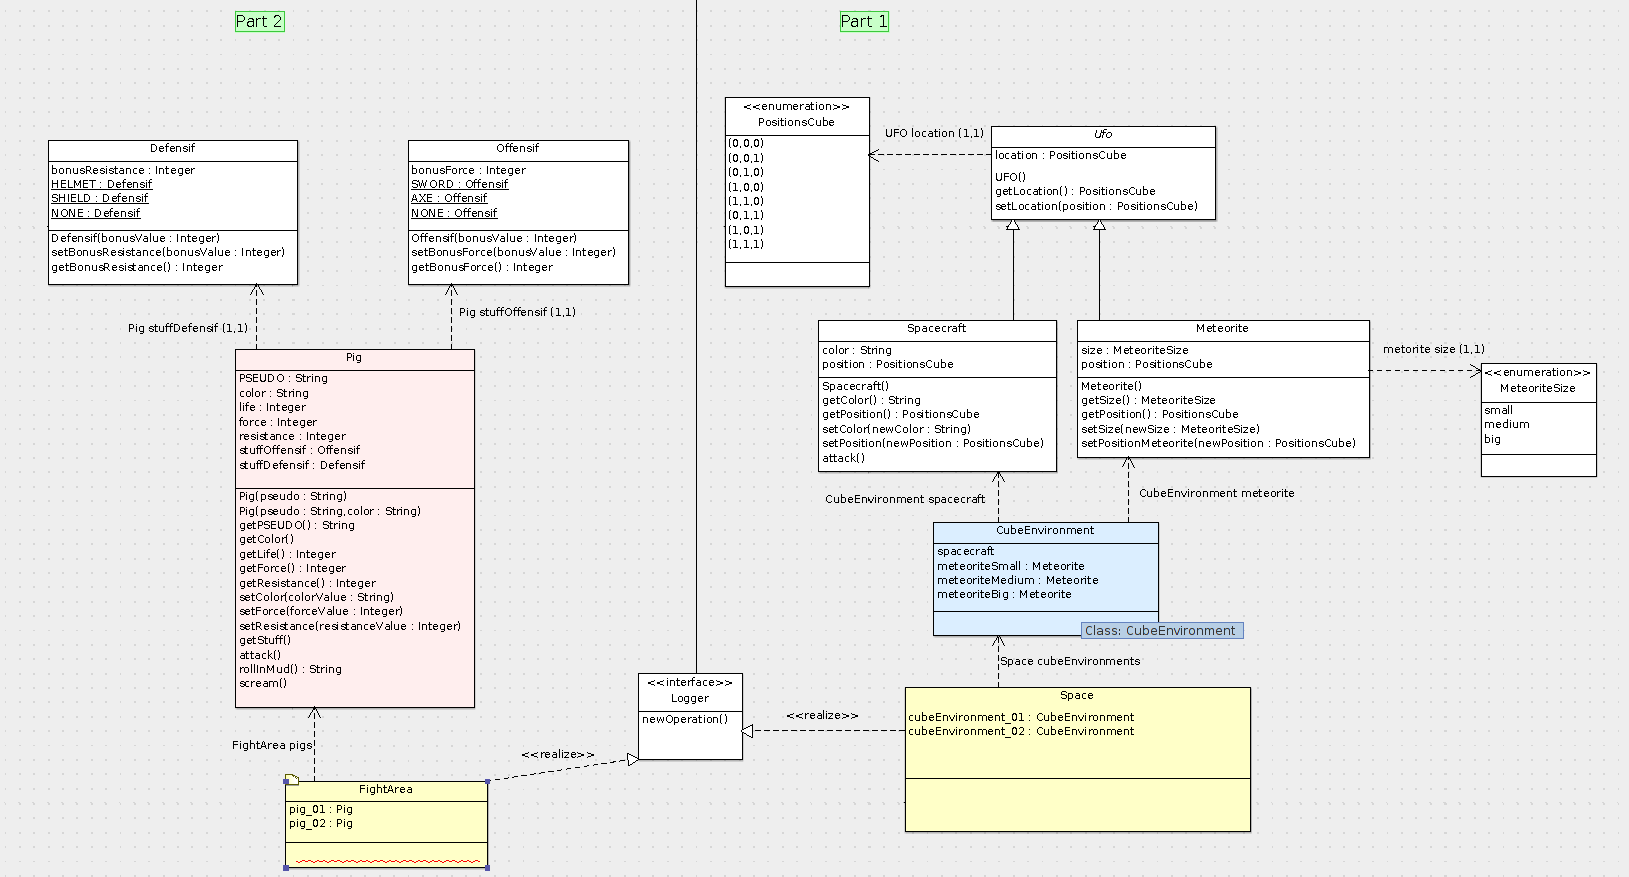
\includegraphics[width=450pt]{../../Images/UMLdiagramme.png}

Since you can't see anything on this screenshot, there are bigger screenshots below.

Blue classes are abstract classes.\\
Green classes are interface.\\
Pink classes are enumeration.\\
Purple classes are exception.\\
Yellow classes are the two main classes from the 2 different parts of the game.\\

\begin{figure}
  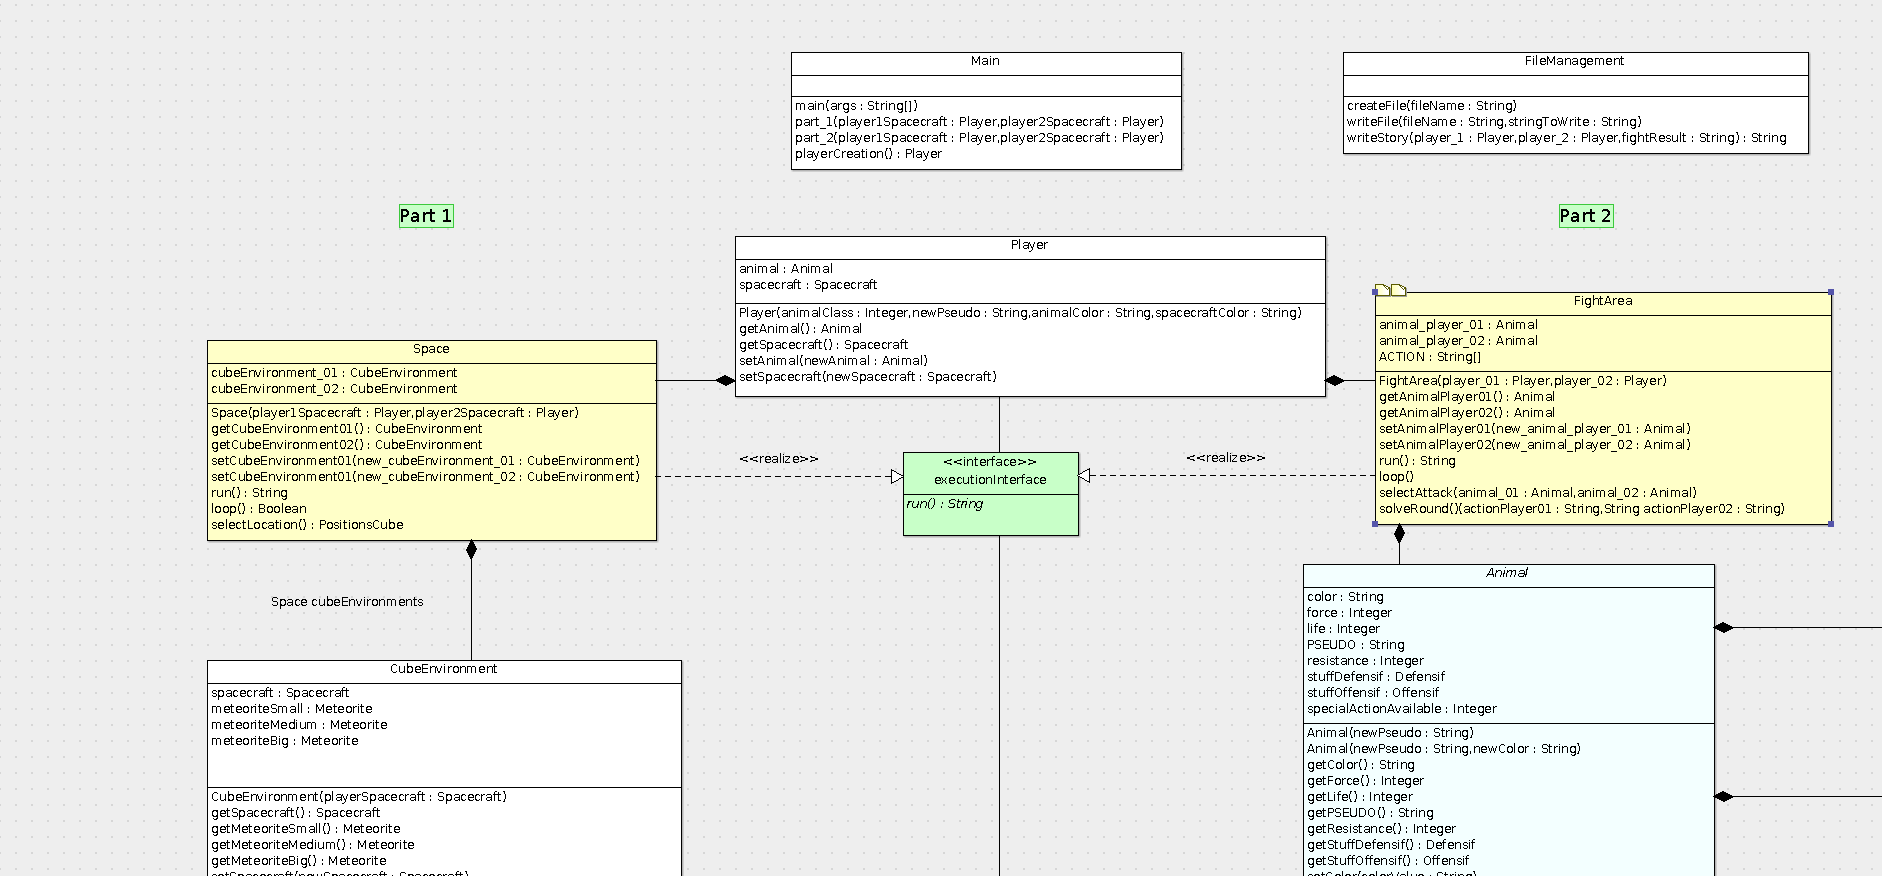
\includegraphics[width=460pt]{../../Images/1_1-2_1.png}
  \caption{\small left screenshot 1}
  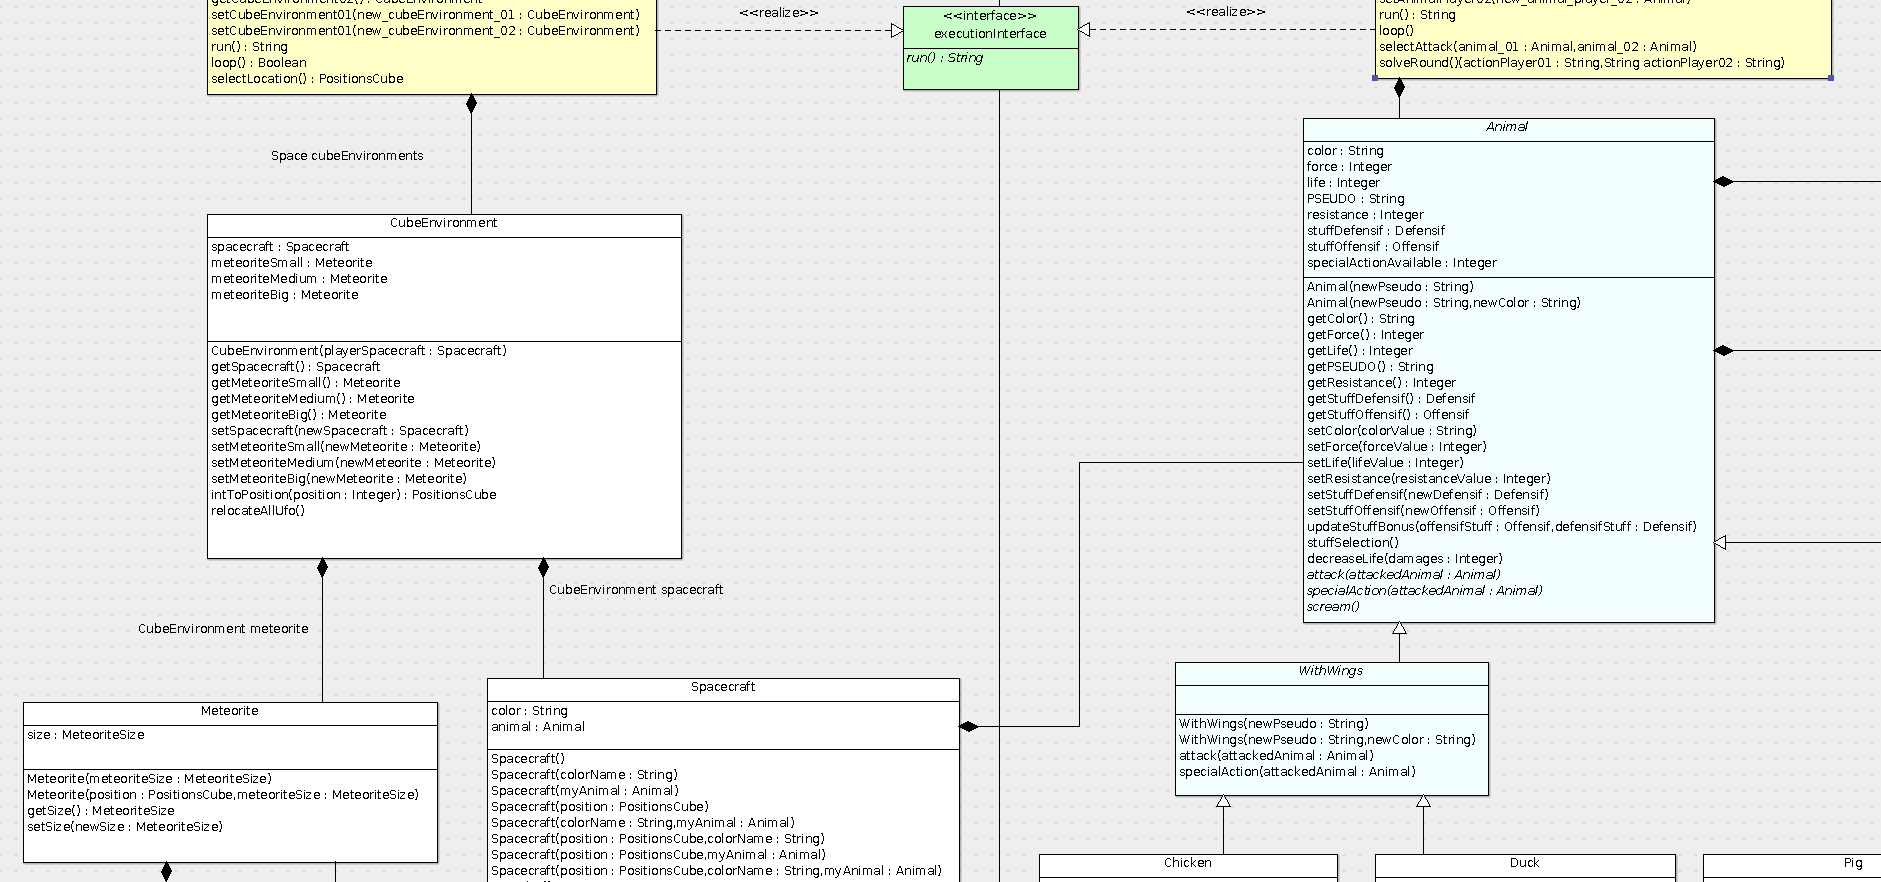
\includegraphics[width=460pt]{../../Images/1_1-1_2-2_2.png}
  \caption{\small left screenshot 2}
  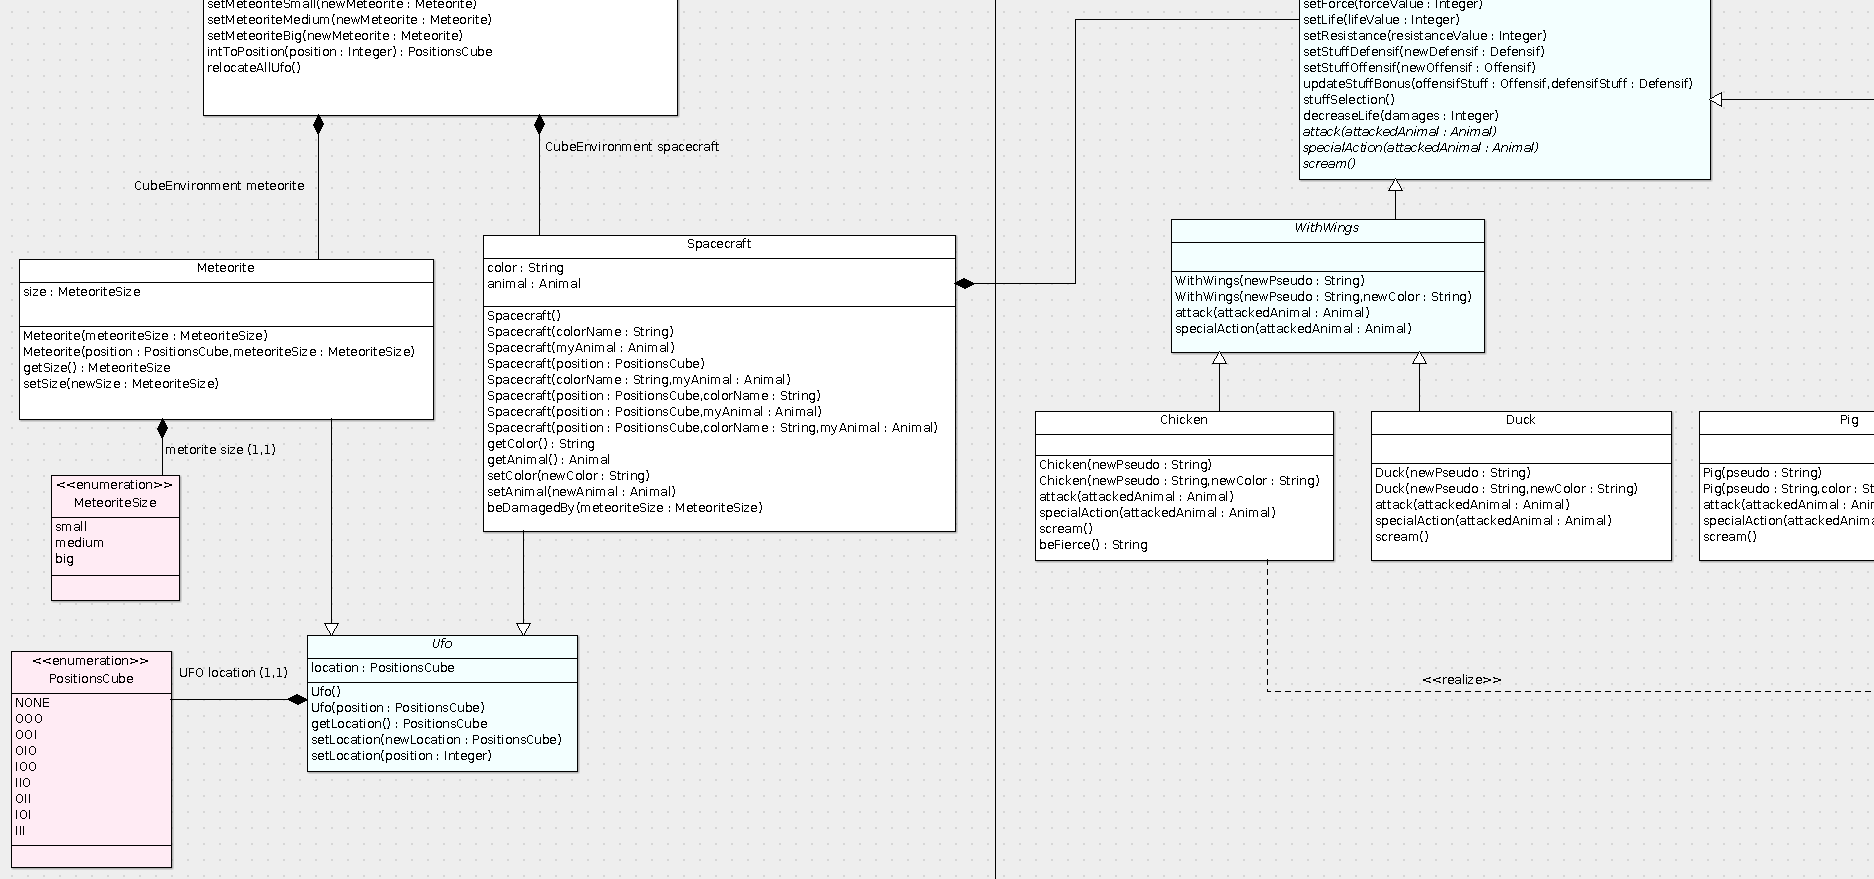
\includegraphics[width=460pt]{../../Images/1_2-2_3.png}
  \caption{\small left screenshot 3}
\end{figure}

\begin{figure}
  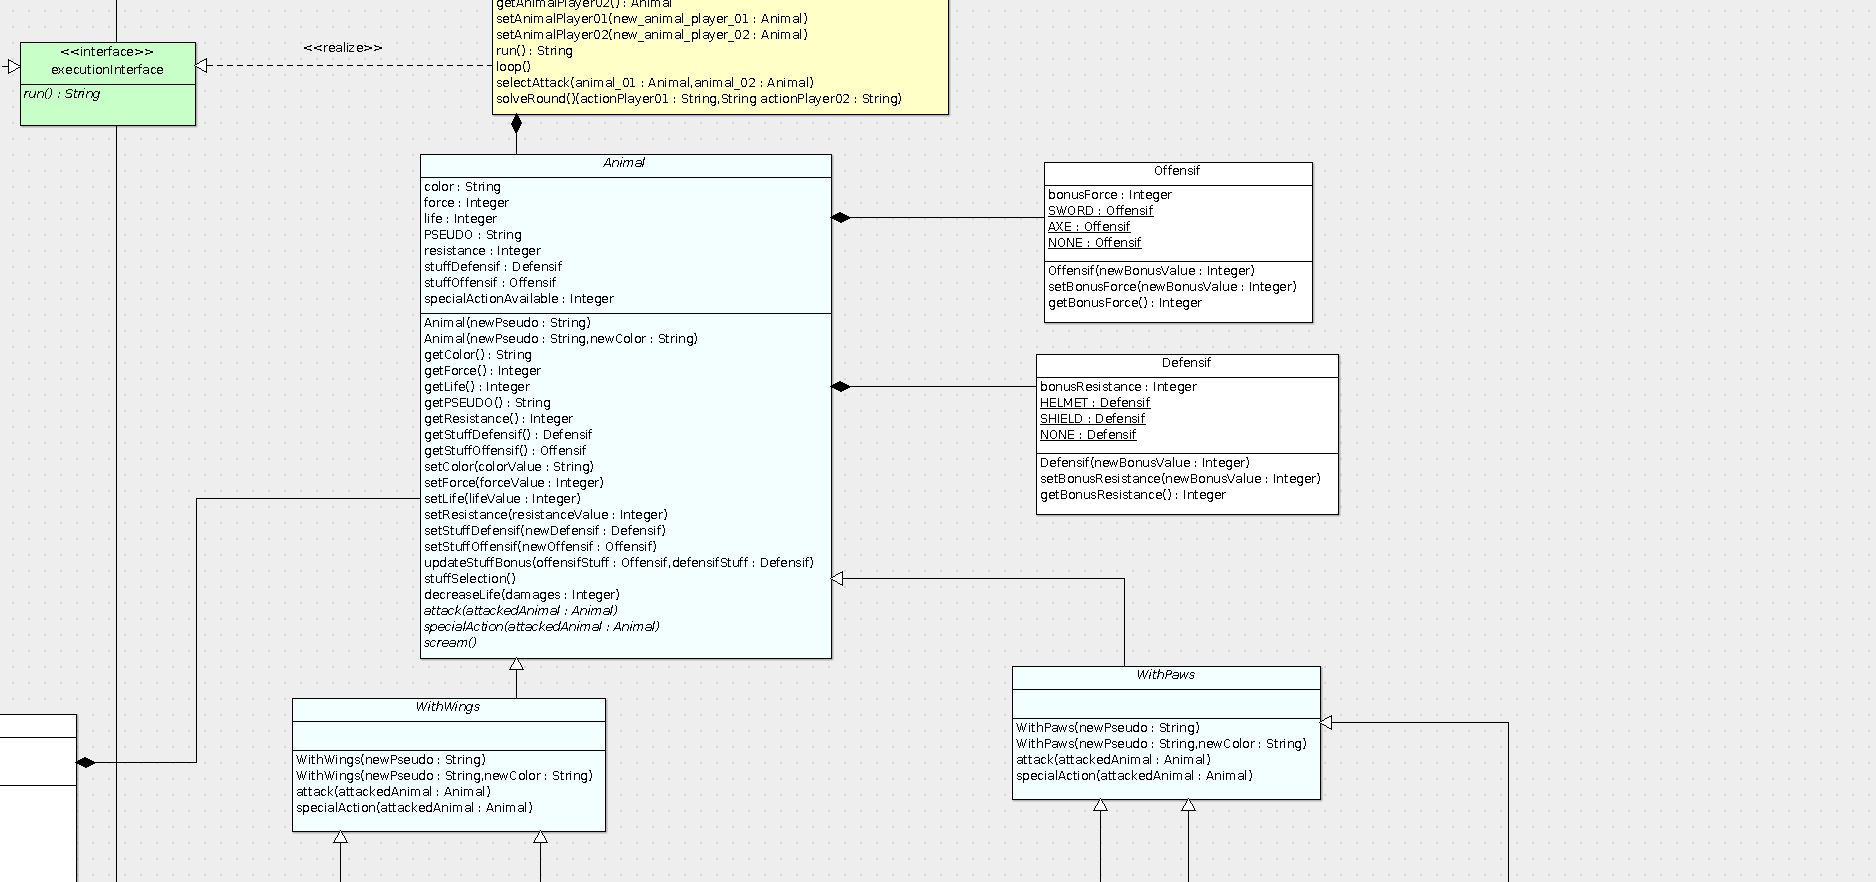
\includegraphics[width=460pt]{../../Images/2_2-3_2-3_3.png}
  \caption{\small right screenshot 1}
  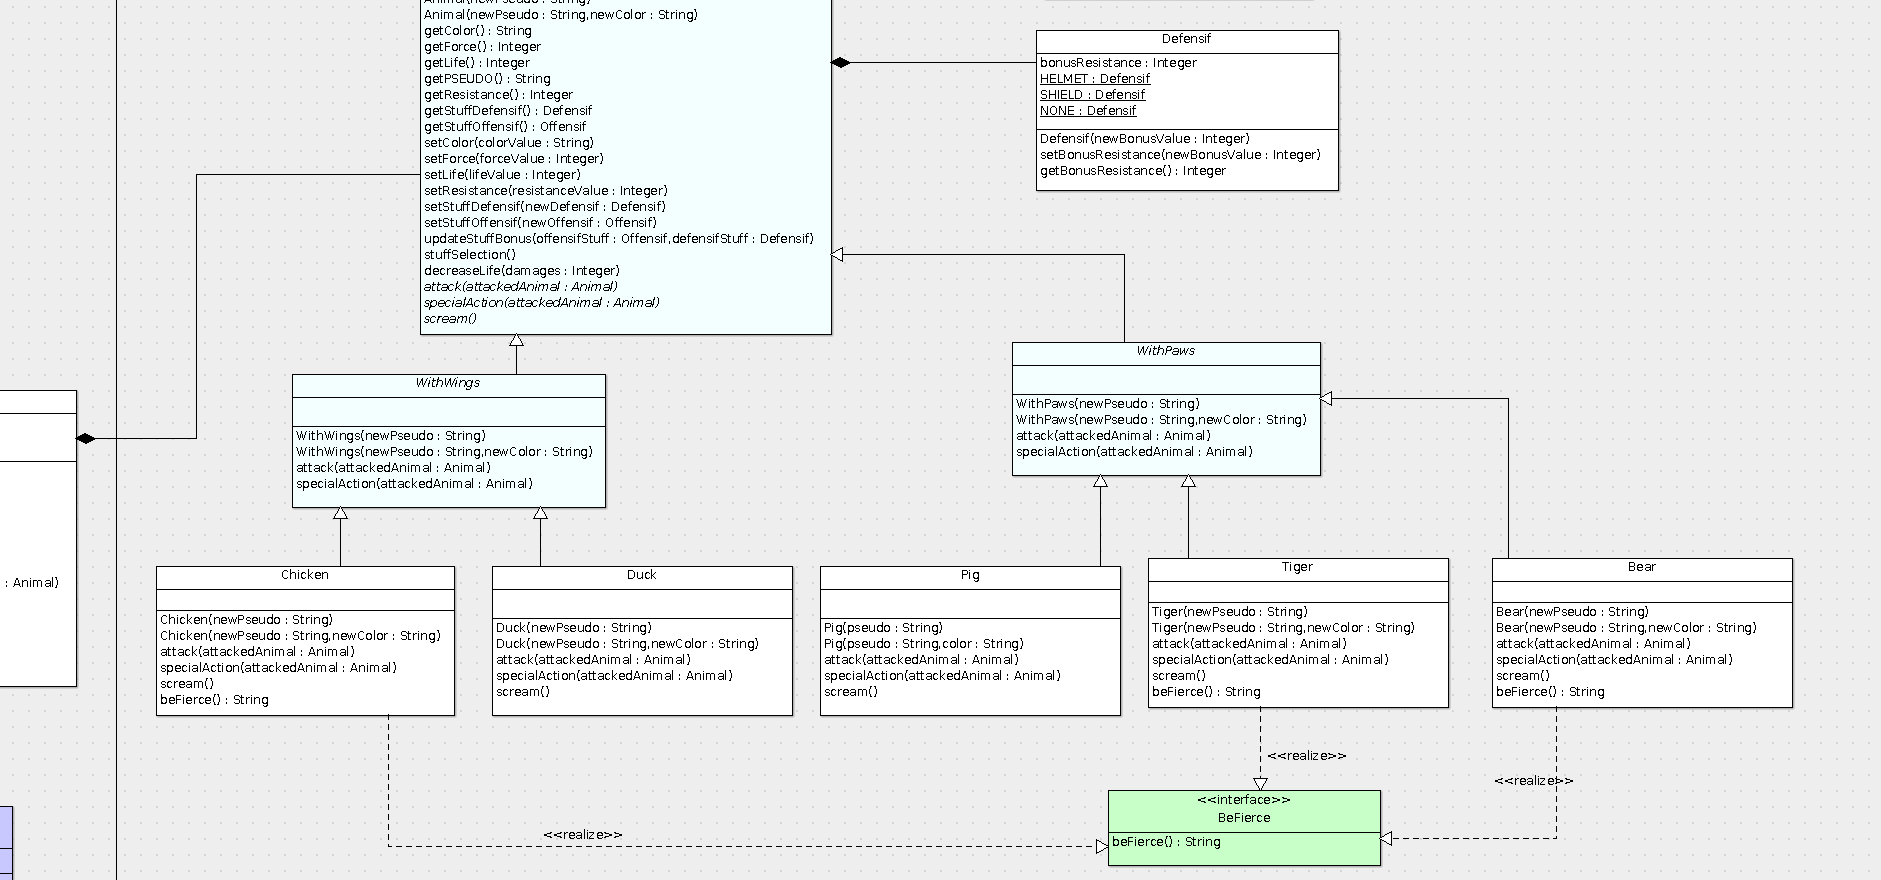
\includegraphics[width=460pt]{../../Images/2_3-3_3.png}
  \caption{\small right screenshot 2}
\end{figure}


% ==========================================================================================
\section{Organisational part: package description}

We created package to organize our project. 
The main package which contains the main classes is called spacePigFighterPackage.

\subsection{spacePigFighterPackage}

This is the main package. It contains the following classes:
\begin{itemize}
 \item Main
 \item Space
 \item FightArea
 \item ExecutionInterface
\end{itemize}

\subsection{fileManagementPackage}

This package contains all classes needed to interact with files. It contains the following class:
\begin{itemize}
 \item FileManagement
\end{itemize}

\subsection{playerPackage}

This package contains all classes needed to create player. It contains the following class:
\begin{itemize}
 \item Player
\end{itemize}

\subsection{cubeEnvironment}

This package contains all classes needed to create space environment. It contains the following class:
\begin{itemize}
 \item CubeEnvironment
\end{itemize}

\subsection{spaceObjects}

This package contains all classes needed to manage space objects. It contains the following classes:
\begin{itemize}
 \item UFO
 \item PositionsCube
 \item Meteorite
 \item MeteoriteSize
 \item Spacecraft
 \item PositionException
\end{itemize}

\subsection{animalPackage}

This package contains all classes needed to manage animal. It does not contain stuff classes. It contains the following classes:
\begin{itemize}
 \item Animal
 \item WithPaws
 \item WithWings
 \item Bear
 \item Chicken
 \item Duck
 \item Pig
 \item Tiger
 \item BeFierce
\end{itemize}

\subsection{stuff}

This package contains all stuff classes. It contains the following classes:
\begin{itemize}
 \item Offensif
 \item Defensif
\end{itemize}






% ==========================================================================================
\section{Technical part: class description}

This part contains a brief description of all project classes.

\subsection{Main}

This class contains the main functions:

\begin{itemize}
 \item main : main function that calls all the following functions.
 \item playerCreation : function that create the 2 players.
 \item part\_1 : function that runs game part 1.
 \item part\_2 : function that runs game part 2.
\end{itemize}


\subsection{FileManagement}

This class contains all useful functions to save the game story in a file. 
We chose to put them in a class in order not to overload the Main class.

\subsection{Player}

We created a Player class that keeps all information about each player. 
That is to say that a player contains a spacecraft and its animal.
It is from this class that we can access all information at any time and everywhere in our code.

\subsection{The 2 main classes of the game}

We created 1 class for each part of the game. 
It is from these 2 classes that each part is run.
They both implements the executionInterface interface.

\subsubsection{ExecutionInterface interface:}

This interface has only one function: \textit{run()}. 
We decided to create this interface in order to create a name convention for the function which runs each part of the game.
By doing this, the Main class won't change, it will always call the \textit{run()} function of each class even if each class change.

\subsubsection{Space class:}

It is composed by 2 CubeEnvironments created thanks to the 2 Players.
It has 3 main functions : 
\begin{itemize}
 \item run() : main function from the interface, it runs all game part 1.
 \item loop() : it runs the main loop while no spacecraft has been found, each player select a location en try to guess spacecraft postition.
 \item selectLocation(): it return the position selected by a player.
\end{itemize}

\subsubsection{FightArea class:}

It is composed by 2 Animals created thanks to the 2 Players and a list of special actions.
It has 4 main functions : 
\begin{itemize}
 \item run() : main function from the interface, it runs all game part 2.
 \item loop() : it runs the main loop while no dead animal has been found, each player select an action to do.
 \item selectAttack(): it allows a player to select an action for its animal to do.
 \item solveRound(): this function manage special actions.
\end{itemize}

\subsection{Part1}

\subsubsection{CubeEnvironment class}

We thought the space environment in a particular way. 
Indeed, we assimilate it to 2 cubes, 1 for each player. That's why the Space class is composed of 2 CubeEnvironment.
Each cube is composed of a spacecraft and 3 meteorites. 
They can be located to 8 different positions that correspond to each corner of the cube.\\
\\
During the 1st part of the game, each player try to find the location of the other one's spacecraft.
Of course he has to avoid meteorites that decrease the life. 
Once one player find the other one, part 2 of the game is started.

\subsubsection{UFO class}

It is an abstract class. 
It was created in order to manage position of both meteorites en spacecrafts.
That's why Meteorite class and Spacecraft class both extends UFO abstract class.\\
\\
To manage location, an UFO has an attribute \textit{location}.
We also created function which make us be able to manage location.
Constructor was overloaded in order to create a UFO default position (000) or take the position in parameter.

\subsubsection{PositionsCube enumeration}

This enumeration enumerates all available positions in a cube. 
These positions match each corner of the cube.
They are coordinates.

\subsubsection{Meteorites}

There are 3 meteorites in each cube. 
A Meteorite has size which can be one from the MeteoriteSize enumeration.
The size impact the amount of life to withdraw to an animal if a player collides a meteorite.

\subsubsection{MeteoriteSize}

This enumeration enumerates all existing meteorite size.

\subsubsection{Spacecraft}

There is one spacecraft in each cube.
Spacecraft class has a color and an Animal.
The spacecraft can be damaged by a meteorite.
A damaged spacecraft means its animal life decreases.

\subsection{Part2}

\subsubsection{Animal class}

It is an abstract class.

\subsubsection{WithWings class}

It is an abstract class which extends animal class.
It overrides \textit{attack()} function to caracterize it by the way the animal attack (with paws or with wings).

\subsubsection{WithPaws class}

It is an abstract class which extends animal class.
It overrides \textit{attack()} function to caracterize it by the way the animal attack (with paws or with wings).

\subsubsection{Bear class}

Bear is an animal with paws. That's why it extends WithPaws abstract class.
It overrides \textit{attack()}, \textit{specialAction()} and \textit{scream()} functions.
Since Bear is a fierce animal, it implements BeFierce interface and overrides \textit{beFierce()} function.

\subsubsection{Chicken class}

Chicken is an animal with paws. That's why it extends WithWings abstract class.
It overrides \textit{attack()}, \textit{specialAction()} and \textit{scream()} functions.
Since Chicken is a fierce animal, it implements BeFierce interface and overrides \textit{beFierce()} function.

\subsubsection{Duck class}

Duck is an animal with paws. That's why it extends WithWings abstract class.
It overrides \textit{attack()}, \textit{specialAction()} and \textit{scream()} functions.

\subsubsection{Pig class}

Pig is an animal with paws. That's why it extends WithPaws abstract class.
It overrides \textit{attack()}, \textit{specialAction()} and \textit{scream()} functions.

\subsubsection{Tiger class}

Tiger is an animal with paws. That's why it extends WithPaws abstract class.
It overrides \textit{attack()}, \textit{specialAction()} and \textit{scream()} functions.
Since Tiger is a fierce animal, it implements BeFierce interface and overrides \textit{beFierce()} function.

\subsubsection{BeFierce interface}

This interface was created to caracterize scream of some animals that are said to be fierce.
It contains 1 function, \textit{beFierce()} function.

\subsubsection{Offensif class}

Each animal has an offensive stuff which gives it a force bonus. 
Offensif class is here to do that.
It has force bonus value and constants that defines existing offensive stuff.

\subsubsection{Defensif class}

Each animal has an defensive stuff which gives it a force bonus. 
Defensif class is here to do that.
It has force bonus value and constants that defines existing defensive stuff.


\subsection{Set the game}

\begin{itemize}
 \item set Player class for each player.
 \item set Space class with 2 CubeEnvironment (1 for each player). Each CubeEnvironment is set with 3 meteorites and 1 spacecraft.
 \item set FightArea class with 2 pigs. Each pig is initialized with stuff selected by the player.
\end{itemize}


\section{Encountered difficulties}

\subsection{Special action}

Special actions are very different. So we had to think our code so that it would be able to welcome each special action.
We had to modify our code a little bit and to add the \textit{solveRound()} function from FightArea. 

\subsection{Exception}

We created an exception. We had difficultie because it was the first time and we didn't undertand exception very well.
Now we do !



\chapter{Conclusion}
Le projet est cool.
%--- End generated contents ---

% Index
\backmatter
\newpage
\phantomsection
\clearemptydoublepage
\addcontentsline{toc}{chapter}{Index}
\printindex

\end{document}
